\section{Arquitetura de sistema}

A arquitetura do sistema desenvolvido pela equipe Oshkosh pertence a classe de
arquitetura de camadas, onde cada camada depende dos dados das camadas
inferiores, não das superiores. Apesar de citado como característica comum
em sistemas de camadas, no artigo do grupo \citep{chen2009terramax}, as
dependências não necessariamente são de cima para baixo. A arquitetura de três
camadas, estado da arte das arquiteturas robóticas, utilizada por diversos
sistemas autônomos, como o AUV Phoenix \citep{gat1991reliable} e o veículo
Stanley \citep{montemerlo2006winning}, pode possuir dependências no estilo
``top-down'' ou interdependência entre camadas.

Essa arquitetura apresenta a grande vantagem de ser flexível e
modular, já que o desenvolvimento de cada camada não depende das outras e as
dependências podem ser simuladas através de objetos \textit{mock}. Com isso,
cada equipe pode trabalhar em sua especialidade, otimizando o tempo e
aumentando a qualidade dos algoritmos desenvolvidos em cada função. Vale
ressaltar que, ao fim do desenvolvimento de cada subsistema, o sistema deverá
ser integrado, portanto o protocolo de comunicação entre camadas e a
plataforma/framework de integração é crucial nesse tipo de arquitetura.

São apresentados sete sistemas~\ref{fig:camadas}: 

\begin{enumerate}
  \item \textit{System Control and User Interface} - normalmente encontrado na
  literatura como \textit{Mission Control System}, ou planejamento de
missão (\textit{Mission Planning}) ou planejamento de tarefas (\textit{Task
Planning}). Como definidpo em \cite{fryxell1996navigation}, o controle de
missão é um sistema que permite ao operador definir as missões de um veículo em
linguagem de alto nível, provê ferramentas adequadas para converter planos em
Programas de Missões que podem ser verificados e executados em tempo real, e
permite ao operador saber o estado da missão enquanto esta é executada, e
modificá-la se for necessário.

  \item \textit{Autonomous Behavior} - é a parte que compõe a autonomia do robô,
  responsável pelo planejamento de trajetórias, e gerenciamento dos
  comportamentos do robô.
  
  \item \textit{Vehicle Management} - camada com os algoritmos de controle
  (controle de posição, estabilidade, velocidade,e  outros).
  
  \item \textit{Perception} - camada que possui os algoritmos de percepção, como
  detecção de obstáculos, detecção da via, detecção de tráfego, detecção de
  faixas, e outros.
  
  \item \textit{Sensor} - \textit{drivers} de sensores, usados para os
  algoritmos de percepção, como câmeras, LIDAR, e outros.
  
  \item \textit{Vehicle Status and Navigation} - sensores para o sistema de
  controle, como posição, velocidade, aceleração e estado do veículo.
\end{enumerate}
 
\begin{figure}[!ht]
\centering
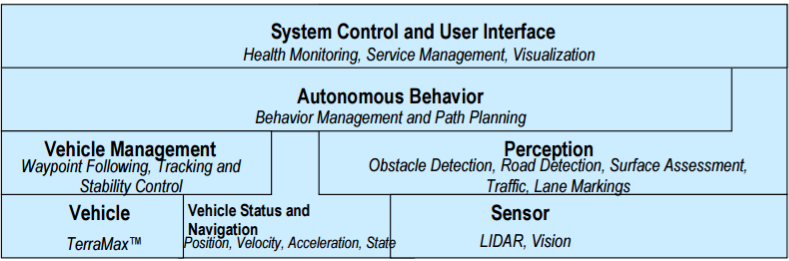
\includegraphics[width=\columnwidth]{figs/camadas.jpg}
\caption{Arquitetura de camadas do veículo TerraMax}
\label{fig:camadas}
\end{figure}

O autor não se aprofunda, no artigo, em como é realizada a integração entre as
camadas, isto é, como a informação e dados transitam, porém ele utiliza
uma terminologia comumente presente na literatura: ``serviços'' e
``\textit{publisher-subscriber}''. Frameworks como o ROS, estado da arte,
possibilitam a utilização de ambos os tipos de comunicação.

\begin{itemize}
  \item \textit{serviço ou cliente-servido} -  componentes falam diretamente
  com outros componentes. As vantagens deste protocolo são: definição prévia da
  interface; e é uma abordagem distribuída para comunicação, já que não há um
  módulo central que distribui os dados. Uma desvantagem deste protocolo é o
  \textit{overhead}, que é significativo se muitos componentes precisam de uma
  mesma informação.
  
  \item \textit{publish-subscriber} - um componente publica dados e qualquer outro componente
pode subscrever (ouvir) a esse dado. Normalmente, há um processo central que
roteia os dados entre \textit{publish} e \textit{subscriber}. Em uma arquitetura
típica, um componente pode publicar e subscrever a vários tipos de informações.
As vantagens desse protocolo de comunicação são: simplicidade e pouco
\textit{overhead}; ideal quando não se sabe quantos componentes diferentes
necessitarão dos dados (como em muitas interfaces); componentes não ficam
sobrecarregados em caso de múltiplos pedidos de um mesmo dado. Suas principais
desvantagens são: difícil depuração de código, pois normalemente a sintaxe da
mensagem está escondida em uma simples \textit{string} (uma \textit{lista}
pode ser enviado como \textit{string} e o componente subscritor retraduz);
utilização de um servidor central que distribui as mensagens (recebe dos
\textit{publishers} e envia aos \textit{subscribers}), o que pode criar um único
ponto de falha e sobrecarga.
   
\end{itemize}

As camadas de \textit{System Control and User Interface} e \textit{Autonomous
Behavior} se comunicam através de mensagens do tipo serviço, enquanto que os
dados da camada \textit{Sensor} são publicados para as demais camadas.

\subsection{Autonomous Behavior}
